\documentclass[preprint,12pt,authoryear]{elsarticle}

\usepackage{amsmath,amssymb,amsthm}
\usepackage{booktabs}
\usepackage{array}
\usepackage{tabularx}
\usepackage{graphicx}
\graphicspath{{./}{figures/}}
\usepackage{enumitem}
\usepackage[colorlinks=true,urlcolor=blue,linkcolor=blue,citecolor=blue]{hyperref}
\emergencystretch=3em
\setlength{\tolerance}{2000}

\newtheorem{proposition}{Proposition}
\newtheorem{corollary}{Corollary}
\newcommand{\pos}[1]{\left[#1\right]_+}
\newcommand{\dconv}{\Delta b_{\mathrm{conv}}}
\newcommand{\Ups}{\Upsilon_c}
\newcommand{\Eceil}{E_{\mathrm{ceil}}}
\newcommand{\Acmin}{A_c^{\min}}
\newcommand{\tconv}{\tau_{\mathrm{conv}}}

\journal{Ecological Modelling}

\begin{document}

\begin{frontmatter}

\title{Rising biocapacity total can mask ecological-capital land drawdown: a two-land model}

\author[1]{Amin Abaee\corref{cor1}}
\ead{amin_abaee@ut.ac.ir}
\cortext[cor1]{Corresponding author. \href{https://orcid.org/0000-0002-0019-1842}{ORCID: 0000-0002-0019-1842}.}
\affiliation[1]{organization={Independent Researcher}, city={Tehran}, country={Iran}}

\begin{abstract}
\footnotesize
Biocapacity is reported as an aggregate, despite the wide differences in yield and regeneration among its constituent land types. A rising total can conceal a change in land composition, but it cannot by itself establish that a physical stock has declined. We examine this measurement problem with a two-land model that separates fast-provisioning land from ecological-capital land and allows delays in regeneration and population response. When the supply available to people falls below demand, the model transfers land from the capital class to the fast-provisioning class. If fast land contributes more annual biocapacity per hectare, that transfer raises total model biocapacity while capital-land area falls.

In a fixed-demand comparison—with capital quality at its maximum, debt and technology boost switched off, and restoration disabled—the reduced balance relation has at most one feasible point. It meets the minimum-area boundary at a baseline demand ceiling of about $1.14$\,gha. This branch has no fold or hysteresis, and its slowest return rate stays nonzero, so there is no critical slowing down on that branch. These are properties of the reduced comparison, not claims of path independence in the full model. Above the ceiling, capital-land area approaches its minimum. When the shortfall closes, one-way conversion stops; without restoration, the lower area persists but does not keep declining. In a representative simulation, capital-land area falls $46.2\%$ and its modeled contribution falls $51.7\%$, while total model biocapacity rises $39\%$. These are conditional model results, not measurements of global physical stocks.

In the National Footprint and Biocapacity Accounts (NFA), Edition 2026 (1961--2023), total world biocapacity account value rises $24.9\%$, while biocapacity per person falls $52.7\%$ and the production footprint per person rises $16.7\%$. Cropland contributes $24.06$ percentage points to the total change; Forest biocapacity subtracts $5.95$ points, and built-up land adds $7.44$ as an accounting class. No comparable global physical-stock series was assembled, so we report no physical-stock composite or global decline finding. The SI specifies requirements for such a comparison; it is not an inventory. These results show why component values should accompany aggregate totals.
\end{abstract}

\begin{keyword}
\footnotesize
biocapacity \sep ecological footprint \sep land-use conversion \sep aggregation \sep identifiability \sep critical slowing down \sep delay differential equations \sep carrying capacity
\end{keyword}

\end{frontmatter}

\section{Introduction}\label{sec:intro}

Ecologists use \emph{carrying capacity} to describe the population a resource base can sustain. Because it is difficult to estimate, many models treat it as a fixed ceiling \citep{Cohen1995}. Yet when use outpaces renewal, it may alter the resources that support future production—and with them, the population the resource base can sustain. We ask a narrower measurement question: can total biocapacity rise while a productive land class loses area?

The National Footprint and Biocapacity Accounts (NFA) report biocapacity as annual biological supply and the Ecological Footprint as annual demand on biologically productive area. Both use global hectares (gha): hectares adjusted to the world's average biological productivity for a given year, with the annual basis implicit \citep{GFNStandards2009,GFNGuidebook2019}. Because each account value combines area and productivity, a change in the total cannot tell us whether yields changed, more area entered production, or the mix of land classes shifted. Composite-indicator research calls this \emph{compensation}: gains in one component can offset losses in another \citep{Nardo2008,Becker2017,Fischer2022}. Related critiques examine how the Ecological Footprint should be interpreted \citep{Blomqvist2013,GiampietroSaltelli2014,vdBerghGrazi2015,Galli2016}. The aggregate remains useful, but it is most informative alongside its component values.

Many human--environment models summarize environmental change as a single stock or overall balance. Examples include the World3 system \citep{Meadows1972,Meadows1974,Meadows2004}, models of Easter Island \citep{BranderTaylor1998,Anderies2000}, and coupled Earth-system frameworks \citep{Motesharrei2016,Donges2017,CalvinBondLamberty2018,HendersonLoreau2018}. Other work asks whether human carrying capacity is fixed, variable, or useful as a concept \citep{Cohen1995,vdBerghRietveld2004,Simon1996,Meyer1994,MeyerAusubel1999,Dasgupta2021}; global demographic assessments often project population separately from environmental constraints \citep{UN2022}. Land-use studies, meanwhile, document conversion of forests, grasslands, and wetlands to cropland \citep{Haberl2007,Krausmann2013,Erb2017}. This literature establishes the relevance of land conversion. The open measurement question is what a single biocapacity total can reveal when land classes differ in yield and regeneration.

An orchard makes the distinction concrete. Imagine fast-provisioning ground, such as cropland or intensively managed systems, beside ecological-capital ground, such as forest, soil, wetland, or long-rotation systems. The first can provide an annual harvest; the second holds assets that support future production and often regenerate more slowly. The harvest is a flow. Trees, soil, and other productive assets are stocks.

In the model, a shortfall can trigger conversion from capital ground to fast-provisioning ground. If fast ground contributes more per hectare in a given scenario, the transfer can raise the current aggregate harvest even as capital-land area falls. Replanting may restore a later crop without replacing mature trees, soil, or other slow-renewing assets. Harvest, regeneration, and population also respond on different timescales, so a stable or rising total can coexist with a shrinking productive base. The orchard illustrates an information limit; it is not evidence that NFA accounts measure global physical stocks or a prediction of ecosystem failure.

We formalize the analogy with two effective land classes: fast-provisioning land and ecological-capital land. The latter groups several real systems into one model class; it is not an NFA category. When a shortfall triggers a transfer from capital land to fast land, total model biocapacity can rise while capital-land area $A_c$ falls—provided fast land contributes more per hectare. This conditional result does not imply that NFA categories map directly to $A_c$ or measure the physical assets in the analogy. Related material-ledger work calls the broader flow--stock masking a \emph{productivity illusion}; we study its composition-specific form \citep{Abaee2026c}.\footnote{The v50 PDF is present at the pinned commit. The checksum manifest lists the v49 article files but omits v50; the README dated 2026-09-19 does not explicitly label v49 or v50; and the v50 TeX header points to the v48 Markdown source.}

An elevator offers a second analogy. A car rated for ten passengers might keep running while carrying fourteen, but the ride itself does not show whether repeated overloading has reduced the cable's safety margin. The analogy separates delivered service from the condition of the asset behind it; it does not predict an inevitable or sudden failure. In the reduced fixed-demand model, the balance curve reaches a specified area minimum without folding back.

We ask three questions. Under what conditions can conversion raise total biocapacity while $A_c$ falls, how long can that pattern last, and what can the total reveal about the area change? Does the modeled drawdown involve a fold, hysteresis, or early-warning signals, or does it follow another path? Finally, what limits drawdown, and what would allow capital-land area to recover?

The paper makes three contributions. First, it develops a two-land model that conserves area, tracks capital-land quality separately, and allows shortfalls to trigger delayed conversion. Second, it derives the condition under which conversion raises total biocapacity and shows why the total cannot identify the land split. It also distinguishes the unique balance point in a reduced fixed-demand comparison from the history-dependent path to that point. Third, it decomposes NFA Edition 2026 account changes and examines a separate crop-area/yield proxy, while clarifying what these data can and cannot establish. We also derive five testable predictions. Parameters are representative rather than fitted, so simulations illustrate conditional mechanisms, not forecasts.

\section{Methods}\label{sec:model}

\subsection{A two-land model with conserved area and a separate quality state}\label{sec:equations}

We divide total bioproductive area $A_{tot}$ among three classes. Fast-provisioning land $A_f$ represents cropland and intensively managed systems. Ecological-capital land $A_c$ groups forest, soil, wetland, and long-rotation systems into one effective class, rather than treating them as a single real land type. Reserve land $A_r$ includes fallow, retired, or not-yet-allocated area. The three areas always sum to $A_{tot}$.

Capital land also has a separate quality state $q\in[0,q_{\max}]$. Quality affects annual biocapacity per hectare, not land area, and follows the logistic growth rule:
\begin{equation}\label{eq:Gc}
G_c(q)=\rho_c\,q\left(1-\frac{q}{q_{\max}}\right),
\end{equation}
We define capital land's annual contribution per hectare as direct yield plus a term linked to quality growth:
\begin{equation}\label{eq:Ups}
\Ups(q)=b_c+b_{G,c}\,G_c(q),
\end{equation}
Here $b_c$ is direct yield, while $b_{G,c}$ converts quality growth into annual account value. The two land classes contribute $Y_f$ and $Y_c$; their sum is total model biocapacity:
\begin{equation}\label{eq:B}
B=Y_f+Y_c=b_f A_f+\Ups(q)\,A_c ,
\end{equation}
The model's $B$ is an annual account-equivalent amount in gha, with the annual basis implicit \citep{GFNStandards2009,GFNGuidebook2019}. Demand is $E=eP$, where $P$ is population and $e$ is the constant footprint per person (gha per person; $\mathrm{cap}$ denotes one person in the equations and tables). The shortfall $S$ is the part of demand not met by the human-available shares of the two land contributions:
\begin{equation}\label{eq:S}
S=\pos{E-\sigma_f Y_f-\sigma_c Y_c},
\end{equation}
The positive-part operator is $\pos{x}=\max(x,0)$; the baseline makes both land contributions fully available ($\sigma_f=\sigma_c=1$). While a shortfall remains, the model transfers capital land to fast-provisioning land at a finite rate:
\begin{equation}\label{eq:uc}u_c=\frac{1}{\tconv}\min\!\left(\frac{S}{b_f},\;A_c-\Acmin\right)\qquad[\mathrm{ha\,yr^{-1}}],
\end{equation}
Here $S/b_f$ is the fast-land area needed to cover the shortfall, $\Acmin$ is the minimum allowed capital-land area, and $\tconv$ sets the conversion timescale. Land moves among classes through one-to-one transfers:
\begin{align}
\dot A_c&=-u_c+R_{rc},\label{eq:Ac}\\
\dot A_f&=u_c+\mu A_r-\eta_f A_f,\label{eq:Af}\\
\dot A_r&=-\mu A_r+\eta_f A_f-R_{rc},\label{eq:Ar}
\end{align}
The maintenance flow $\mu A_r$ moves reserve land into fast use; $\eta_f A_f$ retires fast land to reserve. The model returns reserve land to ecological-capital use only through the surplus-gated restoration flow $R_{rc}$:
\begin{equation}\label{eq:Rrc}
R_{rc}=\chi_r\,A_r\,\pos{B-E},
\end{equation}
These transfers conserve total area; $A_r$ is the remainder after $A_f$ and $A_c$ are specified. Quality responds to its delayed value, while population follows a delayed logistic law \citep{Pearl1925,Hutchinson1948} with carrying capacity $K=\max(B/e,K_{\min})$. The model also accumulates the aggregate deficit $E-B$ as debt, which reduces fast-land yield:
\begin{align}
\dot q&=G_c\big(q(t-\tau_g)\big),\label{eq:q}\\
\dot P&=rP\left(1-\frac{P}{K(t-\tau_p)}\right),\qquad K=\max(B/e,\,K_{\min}),\label{eq:P}\\
b_f&=\big(b_{f0}+T_b(t)\big)\,e^{-\alpha D},\label{eq:bf}\\
\dot D&=\pos{E-B}-\eta D,\label{eq:D}\\
T_b(t)&=\omega_{Tb}\,\frac{\Delta b}{1+e^{-\kappa_w(t-t_{wave})}},\qquad \omega_{Tb}\in\{0,1\}.\label{eq:Tb}
\end{align}
The model distinguishes land area, annual account amounts, and accumulated shortfall. Areas $A_f$, $A_c$, and $A_r$ are measured in hectares; $B$, $E$, and $S$ are annual account amounts in gha, with the annual basis implicit. Debt $D$ is a leaky state driven by the aggregate deficit $E-B$ and is measured in gha\,yr; both $\dot D$ and $\eta D$ are in gha. Debt is an internal model state, not an area or an NFA-reported quantity.

The optional technology boost $T_b$ raises fast-land yield along a bounded logistic curve. It is off in the baseline, figures, and tables, and appears only in the matched comparison in SI~\S S8. The model's dynamic states are $A_f$, $A_c$, $q$, $P$, and leaky debt $D$. Timber liquidation and direct restoration from fast land to capital land are possible extensions, but neither is active in the reported runs (SI~\S S1).

Conversion switches off exactly when the shortfall reaches zero and proceeds at the finite rate set by $\tconv$. Changes in $q$ alter value per hectare without changing area. Reserve replanting can maintain fast land when conversion is inactive; without it, retirement would eventually reduce fast-land area to zero at a no-conversion equilibrium.

Two feedback loops shape the model. First, when fast land contributes more annual biocapacity per hectare than capital land ($b_f>\Ups(q)$), conversion raises $B$ at the margin. Higher $B$ can support a larger population; after the demographic delay, that population may raise demand and produce another shortfall. Maintenance, retirement, and quality change also affect $B$, so the conversion term alone does not determine the total's direction.

Second, a shortfall adds to debt $D$, and repayment draws it down. As debt grows, fast-land yield $b_f$ falls; this can reduce $B$ and deepen the shortfall. Under fixed demand, if the shortfall settles, debt approaches a finite level.

\subsection{Parameters and their status}\label{sec:params}

Table~\ref{tab:params} lists the baseline values and their evidence status. The model compresses forests, soils, wetlands, and other slow-renewing assets into one effective capital-land class, although these systems differ in area, condition, yield, and recovery time. Most parameters are representative rather than fitted. Recovery records also span a wide range: forest biomass reaches about half its reference level after a median of $30$\,yr, collapsed fish stocks after about $5.6$\,yr, and soil organic carbon returns toward a new balance over roughly $17$--$23$\,yr (SI~\S S5.5) \citep{Poorter2016,HutchingsReynolds2004,Neubauer2013,Poeplau2011}. These records provide timescale context. They do not define a global average, estimate $\rho_c$, or determine the model delay $\tau_g$.

Two data-based quantities help describe cropland but do not calibrate the model: the NFA cropland account value per unit area and a separate cereal-yield/cropland-area proxy (SI~\S S5). Neither is a fitted value of $b_f$ or a direct measure of ecological capital, and their boundaries do not map one-to-one onto model fast land. The baseline assumes $b_f-\Ups(q)>0$, so a transfer raises $B$ at that moment. This is a model condition, not an empirical prediction.

\begin{table}[!htbp]
\centering\footnotesize
\renewcommand{\arraystretch}{0.95}
\caption{Baseline parameter values and evidence status. Representative values are effective, lumped quantities; the NFA account/area quotient is descriptive, not a physical-yield measurement. Extension parameters are active only in scenarios specified in this table or the SI. Symbols and units are listed in SI~\S S1.}
\label{tab:params}
\setlength{\tabcolsep}{4pt}
\begin{tabularx}{\textwidth}{@{}>{\raggedright\arraybackslash}p{0.13\textwidth} >{\raggedright\arraybackslash}p{0.2\textwidth} >{\raggedright\arraybackslash}X >{\raggedright\arraybackslash}p{0.26\textwidth}@{}}
\toprule
Parameter & Value & Meaning & Status \\
\midrule
$\rho_c$ & $0.08$\,yr$^{-1}$ & quality regeneration rate of capital land & representative; not fitted \\
$b_{f0}$ & $0.85$\,gha\,ha$^{-1}$ & base fast-land yield per hectare & representative (2026 NFA account value/area quotient $\approx1.045$ in 1961; not a physical-yield measure) \\
$b_c$ & $0.05$\,gha\,ha$^{-1}$ & capital-land direct yield & representative \\
$b_{G,c}$ & $0.8$\,gha\,yr\,ha$^{-1}$ & regeneration-value coefficient for capital land & representative \\
$q_{\max}$ & $1.0$ (dimensionless) & normalized quality ceiling & normalization \\
$\mu$ & $0.06$\,yr$^{-1}$ & cropland maintenance (reserve$\to$fast) & representative \\
$\eta_f$ & $0.05$\,yr$^{-1}$ & fast-land retirement (fast$\to$reserve) & representative \\
$\tconv$ & $1.0$\,yr & conversion time constant & representative \\
$\alpha$ & $0.03$\,gha$^{-1}$\,yr$^{-1}$ & degradation of $b_f$ per unit debt & representative \\
$\eta$ & $0.05$\,yr$^{-1}$ & debt-repayment rate ($>0$) & representative \\
$e$ & $0.55$\,gha\,cap$^{-1}$ & per-capita footprint (constant) & representative \\
$r$ & $0.02$\,yr$^{-1}$ & intrinsic population growth & representative \\
$\tau_g,\ \tau_p$ & $20,\ 25$\,yr & regeneration and demographic delays & representative; $\tau_p$ lumps institutional lags \\
$A_{tot}$ & $2.5$\,ha & total bioproductive area & normalization \\
$\sigma_f,\ \sigma_c$ & $1,\ 1$ (dimensionless) & human-available shares of annual account amounts & baseline ($<1$: reservation extension) \\
$\chi_r$ & $0.10$\,gha$^{-1}$\,yr$^{-1}$ & surplus-gated restoration coefficient & on with endogenous demand; off under frozen demand \\
$\Acmin$, $A_r^{\min}$,\newline $K_{\min}$ & $0.05$\,ha, $0.10$\,ha,\newline $0.02$\,cap & typed floors & domain constraints \\
$\Delta b$, $\kappa_w$,\newline $t_{wave}$ & $1.0$\,gha\,ha$^{-1}$, $0.1$\,yr$^{-1}$,\newline $40$\,yr & technology wave & off in baseline; active only in the matched SI S8 experiment \\
\bottomrule
\end{tabularx}
\end{table}

\subsection{Data and empirical measures}\label{sec:data}

We use the official National Ecological Footprint and Biocapacity Accounts, Edition 2026, results and metadata version 1.0 \citep{Lo2026NFA}. The primary analysis uses complete world observations for 1961--2023 and excludes estimates for 2024--2025. Our 1961--2022 sensitivity uses the same edition and population series, keeping the data vintage constant across both windows.

From the workbook's \texttt{world\_data} sheet, we take total biocapacity $B$ from \texttt{biocap\_total\_gha}, the Global Ecological Footprint of Production $E_{\mathrm{prod}}$ from \texttt{efp\_total\_gha}, and UN PopStat population from \texttt{pop\_1000\_persons}. We convert population from thousands to persons and calculate per-person values from unrounded totals, not the rounded per-person columns. Ratios, indices, and log changes are dimensionless.

We retain the workbook's component labels: Cropland, Grazing land, Forest biocapacity, Fishing grounds, and Built-up land. These are account values, not measurements of biomass, soil condition, wetland extent, fish biomass, or model area $A_c$. Built-up land is an NFA accounting class, not ecological capital. We therefore interpret component movements only as changes in account composition. SI~\S S5 gives variable definitions and endpoint calculations.

As a separate check, we pair OWID's FAOSTAT-derived world cropland-area series (arable land plus permanent crops) with cereal yield \citep{OWIDCereal2026,OWIDCropland2026}. Cereal yield is a limited productivity indicator, not a measure of all-crop output or an NFA yield factor. We scale the proxy to the NFA cropland share of total biocapacity in 1961, calculate $X_t=\hat b_{f,t}A_{f,t}$, and define the remainder as $C_t=B_t-X_t$. This is an assumed account split, not a measured division of physical capital. The remainder absorbs differences in boundaries, categories, and calibration; it is not $\Upsilon(q)A_c$. SI~\S S5 reports the proxy and its calibration sensitivity. We infer no physical-stock trend from it.

To compare total and per-person biocapacity, we use the exact identity $\Delta\ln B=\Delta\ln(B/P)+\Delta\ln P$. This separates scale from per-person change as an accounting matter; it does not identify causes of biocapacity production.

\subsection{Numerical solution}\label{sec:numerics}

We integrate the delay equations with the method of steps and an explicit first-order Euler scheme. The demonstration run and threshold bisection use $\Delta t=0.05$\,yr; drawdown sweeps use $0.1$\,yr, with selected thresholds checked at $0.05$\,yr. The positive-part switch is exact. We enforce $A_c\ge\Acmin$, $A_f\ge0$, $q\in[0,q_{\max}]$, $P,D\ge0$, and $K\ge K_{\min}$. Before each run, $B$ and $q$ are held at their initial values throughout the longest active delay. Both runs in the controlled technology-wave experiment share the same no-wave history; the wave changes current $B$ and, later, the delayed carrying-capacity input. Because floor-proximity values depend on time step and tolerance, we report bands rather than sharp thresholds. All reported trajectories use delayed quality, $G_c(q(t-\tau_g))$. SI~\S S3 compares the current-quality alternative; SI~\S S8 gives the matched wave experiment and step-size checks.
\section{Results}\label{sec:results}

\subsection{When conversion raises the total as capital land declines}\label{sec:mask}

For a given capital-land quality level $q$, its annual contribution per hectare, $\Ups(q)$, is a concave quadratic. It peaks at $q^*=q_{\max}/2$; with the baseline parameters, the maximum is $0.066$\,gha\,ha$^{-1}$. The quality-related term contributes $0.016$ of that value, while direct yield contributes $0.05$\,gha\,ha$^{-1}$; the direct-yield component is larger in this case.

Conversion changes the aggregate according to the gap between the annual account contribution of one fast-land hectare and the effective value of one capital-land hectare. We call this gap the \emph{composition diagnostic}:
\begin{equation}\label{eq:dconv}
\dconv(q,D)=b_f(D)-\Ups(q).
\end{equation}
At baseline, $\dconv$ equals $+0.787$, $+0.784$, and $+0.794$\,gha\,ha$^{-1}$ at $q=0.3$, $0.6$, and $0.9$. Each lies in the composition-premium regime ($\dconv>0$), where conversion adds to the aggregate at the margin. At $\dconv=0$ the contribution is first-order neutral; below zero, it is a composition-discount. These labels describe the conversion term only. Maintenance, retirement, quality change, and other flows still determine the net change in $B$. At any given quality level, that contribution changes linearly with $A_c$; it has no interior maximum with respect to area.

\begin{proposition}[Conversion, aggregate change, and what the total can reveal]\label{prop:mask}
Let $T_b\equiv0$, $R_{rc}\equiv0$ and hold $D$ fixed, so that $b_f$ is constant. Along any solution of \eqref{eq:B}--\eqref{eq:q},
\begin{equation}\label{eq:identity}
\dot B=\dconv(q)\,u_c+b_f\big(\mu A_r-\eta_f A_f\big)+b_{G,c}\,G_c'(q)\,A_c\,\dot q .
\end{equation}
\begin{enumerate}[label=(\roman*)]
\item During conversion ($u_c>0$), $A_c$ falls when restoration is off. The conversion component of $\dot B$ is $\dconv(q)u_c$, positive exactly when $\dconv(q)>0$. It determines the sign of net $\dot B$ only if maintenance balances retirement ($\mu A_r=\eta_fA_f$) and quality is unchanged ($\dot q=0$).
\item In the reduced comparison—with fixed demand and debt, baseline availability shares, balanced maintenance and retirement, and no quality change—a positive $\dconv$ makes the shortfall shrink during conversion. The shortfall closes if the balance point is reached before the area floor binds. If the floor binds first, $A_c$ approaches $\Acmin$ and a shortfall may persist. Other active terms in the full model can change this result.
\item At fixed $b_f>0$ and $q$, $B=b_fA_f+\Ups(q)A_c$ supplies one equation for the two land areas. Near an interior state, a small change in $A_c$ can be offset by $\delta A_f=-(\Ups/b_f)\delta A_c$ and $\delta A_r=-\delta A_f-\delta A_c$, preserving both $B$ and total area as long as the land bounds are respected. Thus several nearby allocations can have the same $B$; the aggregate alone does not identify $A_c$. For a finite observed change $\Delta B$, the offset is $\Delta A_f=(\Delta B-\Ups\Delta A_c)/b_f$. It is feasible only if all resulting areas remain within bounds, so the feasible range depends on the starting state. If $A_f$ and $b_f$ are observed independently, the residual $C=B-b_fA_f=\Ups(q)A_c$ identifies their product, not its two factors. An independent observation of $A_c$ would give $\Ups(q)=C/A_c$. A single value of $\Ups$ cannot separate $b_c$, $b_{G,c}$, $\rho_c$, and $q$. Even with informative observations of $q$, it identifies at most $b_c$ and the product $b_{G,c}\rho_c$, not $b_{G,c}$ and $\rho_c$ separately.
\end{enumerate}
\end{proposition}

\begin{proof}
Differentiate \eqref{eq:B} with $b_f$ constant and substitute \eqref{eq:Ac}--\eqref{eq:Af} with $R_{rc}=0$: $\dot B=b_f(u_c+\mu A_r-\eta_fA_f)-\Ups u_c+b_{G,c}G_c'(q)A_c\dot q$, which is \eqref{eq:identity}. (i) Follows from \eqref{eq:identity} with $R_{rc}=0$; when the maintenance--retirement imbalance and quality-growth terms vanish, only the conversion term remains. (ii) Under the reduced-case conditions in the statement, $S=E-B$ and $\dot S=-\dot B=-\dconv u_c<0$ on $S>0$. Since $S$ is bounded below by zero and $A_c$ is bounded below by $\Acmin$, conversion either closes the shortfall or is limited by the floor. (iii) At fixed $b_f$ and $q$, the observation map is linear; an interior feasible point admits the stated small perturbations along a level set of $B$, while finite changes must also obey the area bounds. The residual $C$ identifies only $\Ups(q)A_c$ unless $A_c$ is independently observed; the parameter combination follows from the definition of $\Ups(q)$.
\end{proof}

Figure~\ref{fig:model}a follows the baseline run with demand fixed at $E=0.825$\,gha and restoration off. Initial states are $A_f=0.6$\,ha, $A_c=1.5$\,ha, $A_r=0.4$\,ha, and $q=0.9$. During conversion, model biocapacity $B$ rises from $0.594$ to $0.825$\,gha ($39\%$); capital-land area falls from $1.500$ to $0.808$\,ha ($46\%$), while fast-land area grows from $0.600$ to $0.923$\,ha.

Quality $q$ rises from $0.9$ to $1.0$, moving farther above $q^*=0.5$, where $\Ups(q)$ peaks. Its per-hectare value therefore falls from $0.05576$ to $0.05000$\,gha\,ha$^{-1}$. The modeled capital-land contribution $\Ups(q)A_c$ falls from $0.08364$ to $0.04038$\,gha ($51.7\%$)—more than the $46.2\%$ area decline because value per hectare also decreases. The one-to-one transfers conserve area: $\Delta A_f+\Delta A_c+\Delta A_r=0$.

The adjustment is fastest early and then slows. On the deficit side, the approach to balance is exponential, with slow rate $|\lambda_1|=0.054$\,yr$^{-1}$ and an e-folding time of about $19$\,yr. By year $25$, $98\%$ of the rise in $B$ and $85\%$ of the decline in $A_c$ have occurred ($B=0.820$\,gha, $A_c=0.913$\,ha); by year $50$, $97\%$ of the area decline is complete. At the reported numerical resolution, $\dot B>0$ and $\dot A_c<0$ together for about $149$\,yr.

Reserve adjustment creates the long tail. As fast land retires to reserve, its contribution falls and a small shortfall reappears. Conversion then continues until $A_r/A_f=\eta_f/\mu$. The duration is not a fixed horizon: the slow rate $\lambda_1$ sets its timescale, while $\dconv$ and the initial shortfall affect its size (SI~\S S2.2).

The aggregate has a clear identification limit: $B$ alone cannot show whether $A_c$ is shrinking while another component grows. Independent observations of fast-land area $A_f$ and yield $b_f$ would let us calculate $C=B-b_fA_f$. But $C$ identifies only the capital-land contribution, not its area and per-hectare value separately.

We call a trajectory with rising $B$ and falling $A_c$ a \emph{composition mask}. A related but distinct pattern is the \emph{liquidation mask}, in which demand $E$ stays fixed while $A_c$ falls. The first compares aggregate biocapacity with land area; the second compares demand with land area. They can occur together, but neither implies the other. The diagnostic $\dconv$ gives the sign of conversion's marginal contribution, not necessarily the net change in $B$ when other terms are active; a liquidation mask does not require $\dconv>0$. Observing $B$, $E$, and $A_c$ distinguishes their defining patterns. Here, “liquidation mask” names a trajectory; it is not the optional timber-liquidation extension, which is off in every reported run.

\begin{figure}[!htbp]
\centering
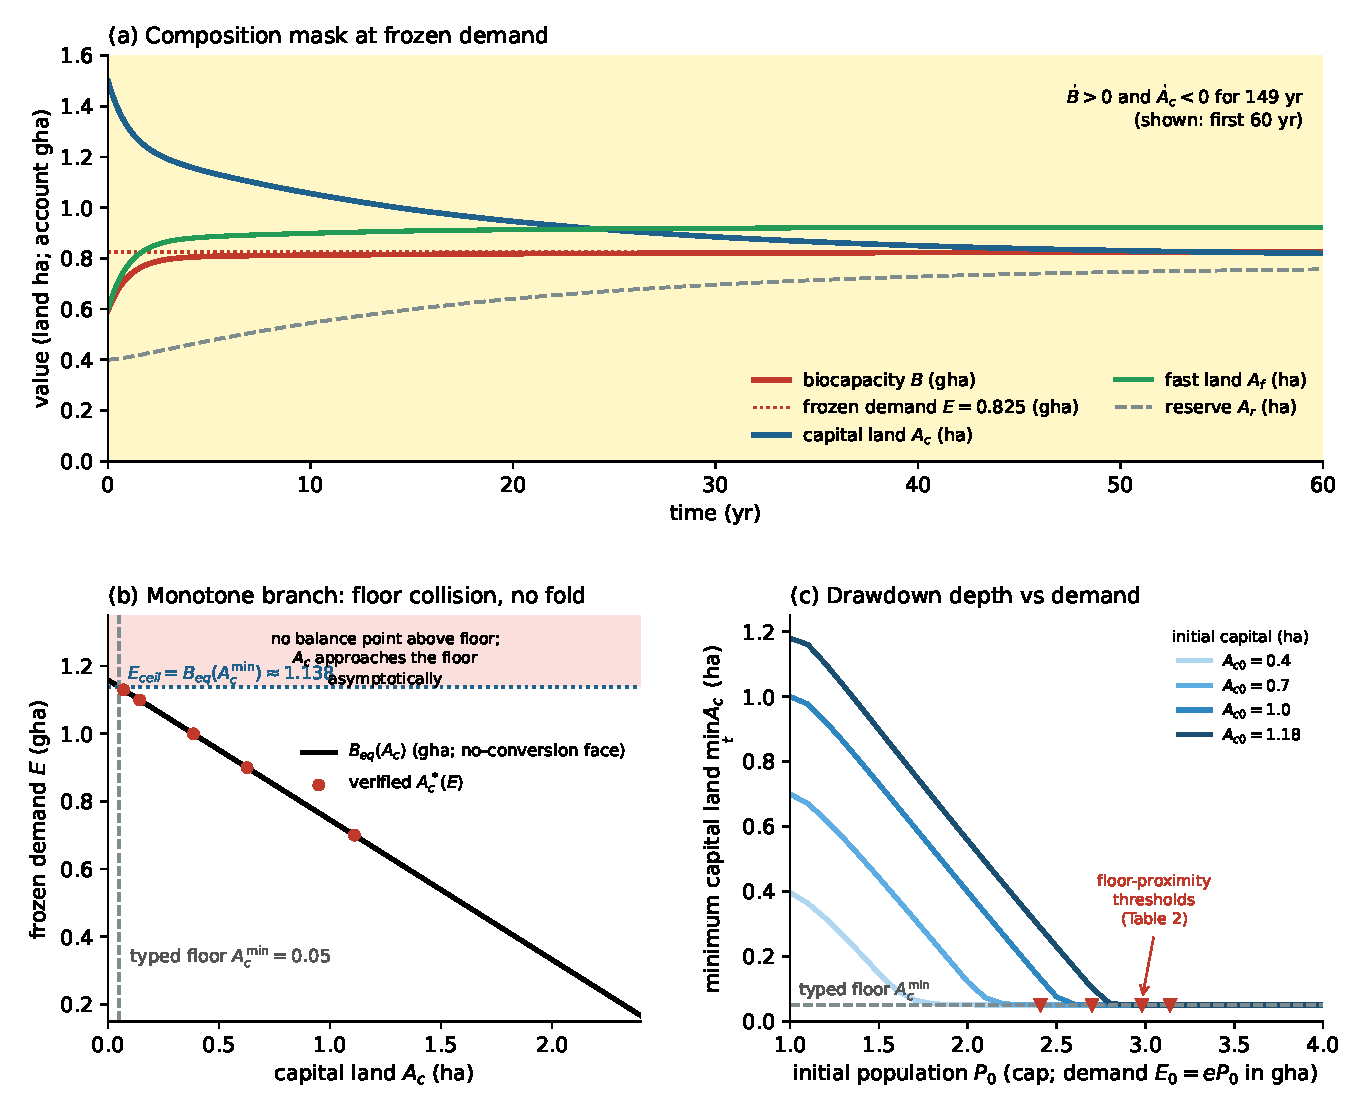
\includegraphics[width=\textwidth]{fig1_model_dynamics}
\caption{Baseline model results (Table~\ref{tab:params}). Account amounts $B$ and $E$ are in gha, land areas are in ha, and population is in cap. (a) Frozen demand ($E=0.825$\,gha), restoration off, and initial conditions $A_{f0}=0.6$\,ha, $A_{c0}=1.5$\,ha, and $q_0=0.9$. $B$ rises from $0.594$ to $0.825$\,gha as $A_c$ falls from $1.500$ to $0.808$\,ha and $A_f$ rises from $0.600$ to $0.923$\,ha. Shading marks the interval with $\dot B>0$ and $\dot A_c<0$ (about $149$\,yr; only the first $60$\,yr are shown). Within $25$\,yr, $98\%$ of the rise in $B$ and $85\%$ of the fall in $A_c$ occur. (b) Fixed-demand balance relation $B_{eq}(A_c)$; the listed balance areas are $A_c^*(E)=1.110$, $0.626$, $0.385$, $0.143$, and $0.070$\,ha at $E=0.70$, $0.90$, $1.00$, $1.10$, and $1.13$\,gha. The curve meets the minimum $A_c=0.05$\,ha at $\Eceil\approx1.138$\,gha; no balance point is admissible at higher demand. (c) Endogenous-demand runs with $\tau_g=20$\,yr, $\tau_p=25$\,yr, and $\chi_r=0.10$\,gha$^{-1}$\,yr$^{-1}$. For each initial area $A_{c0}$, the minimum area reached varies continuously and monotonically with $P_0$ ($E_0=eP_0$). The floor is approached asymptotically. Triangles mark the proximity values in Table~\ref{tab:model}, defined as within $10^{-6}$\,ha of the floor; no discontinuity is observed.}
\label{fig:model}
\end{figure}

\subsection{Fixed demand leads to a minimum-area boundary, not a fold}\label{sec:ceiling}

Once population reaches carrying capacity, $P=K=B/e$ and demand $E=eP$ equals biocapacity $B$; the shortfall then closes. Conversion is therefore transient in the endogenous-population runs. To isolate how the balance point changes with demand, we also fix $E$ and analyze a reduced land system. The constraint $A_c\ge\Acmin$ is a \emph{typed floor}: it protects one land class, not the aggregate.

\begin{proposition}[Balance point, demand ceiling and affine deficit-side dynamics]\label{prop:ceiling}
For this reduced comparison, hold demand at $E$, switch off the technology boost and restoration, set debt $D=0$, and fix quality at $q=q_{\max}$. This quality is the attractor of \eqref{eq:q} for $q(0)>0$. Let $k=\mu/(\mu+\eta_f)$ and
\begin{equation}\label{eq:Beq}
B_{eq}(A_c)=b_{f0}\,k\,(A_{tot}-A_c)+b_cA_c=b_{f0}kA_{tot}-(b_{f0}k-b_c)A_c .
\end{equation}
\begin{enumerate}[label=(\roman*)]
\item With no conversion ($S=0$), reserve-to-fast maintenance balances fast-land retirement. This gives $A_f=k(A_{tot}-A_c)$ and $A_r=(1-k)(A_{tot}-A_c)$, where $k=\mu/(\mu+\eta_f)$. The resulting total is $B_{eq}(A_c)$. If $b_{f0}k>b_c$, this total decreases as $A_c$ increases, so there is at most one balance point $B_{eq}(A_c^*)=E$:
\begin{equation}\label{eq:Acstar}
A_c^*(E)=\frac{b_{f0}kA_{tot}-E}{b_{f0}k-b_c}.
\end{equation}
The algebraic solution is feasible when $B_{eq}(A_{tot})\le E\le\Eceil$, where $\Eceil=B_{eq}(\Acmin)$. It lies above the minimum area exactly when $E<\Eceil$. At lower demand, the algebraic root lies above $A_{tot}$, and every feasible no-conversion allocation already supplies at least $E$.
\item While shortfall is positive and conversion is not yet limited by the minimum-area constraint, the land subsystem is affine in $z=(A_f,A_c)$: $\dot z=Jz+c$, with
\begin{equation}\label{eq:J}
J=\begin{pmatrix}-\tconv^{-1}-\mu-\eta_f & -\mu-\dfrac{b_c}{b_f\tconv}\\[8pt] \tconv^{-1} & \dfrac{b_c}{b_f\tconv}\end{pmatrix},
\qquad \det J=\frac{\mu+\eta_f}{\tconv}\Big(k-\frac{b_c}{b_f}\Big),
\end{equation}
and $\operatorname{tr}J<0$. The matrix does not depend on demand or on the current state. Its determinant is positive exactly when $B_{eq}$ decreases, and its fixed point is the balance point in (i). For $B_{eq}(A_{tot})\le E<\Eceil$, trajectories that remain in this regime approach that point at rates set by the eigenvalues of $J$. For $E>\Eceil$, the balance point would lie below the allowed minimum: $A_c$ approaches $\Acmin$ asymptotically and the shortfall tends to $S^*=E-\Eceil>0$. Thus the reduced balance curve meets the minimum-area boundary; it does not turn back or form a fold. The leading eigenvalue does not approach zero at $E=\Eceil$, and the reduced equilibrium relation has no hysteresis. These conclusions hold under the stated assumptions and do not imply that the realized land allocation is independent of its history.
\item Above the demand ceiling, with degradation active, debt approaches a unique value $D^*(E)$ satisfying $\eta D=E-B_{eq}(\Acmin;D)$, where $B_{eq}(\cdot;D)$ uses yield $b_{f0}e^{-\alpha D}$. This result requires $\eta>\alpha b_{f0}k(A_{tot}-\Acmin)$; the equilibrium debt increases with demand.
\end{enumerate}
\end{proposition}

\begin{proof}
(i) With $S=0$ and $R_{rc}=0$, \eqref{eq:Af} gives $\mu A_r=\eta_fA_f$, hence $A_r/A_f=\eta_f/\mu$ and, with $A_r=A_{tot}-A_f-A_c$, $A_f=k(A_{tot}-A_c)$; substituting into \eqref{eq:B} with $q=q_{\max}$ ($\Ups=b_c$) and $D=0$ gives $B=B_{eq}(A_c)$, and $S=0$ requires $B\ge E$. Strict monotonicity and \eqref{eq:Acstar} follow from $b_{f0}k>b_c$. (ii) On the deficit side $u_c=(E-b_fA_f-b_cA_c)/(b_f\tconv)$ is affine in $z$; substituting into \eqref{eq:Ac}--\eqref{eq:Af} with $A_r=A_{tot}-A_f-A_c$ gives $J$ and a constant vector $c$ by direct differentiation; $\det J$ follows by expansion, and $\operatorname{tr}J=-\tconv^{-1}(1-b_c/b_f)-\mu-\eta_f<0$ for $b_c<b_f$. The fixed point solves $u_c=0$ and $\mu A_r=\eta_fA_f$, i.e.\ it is the balance point. Because $J$ is constant, convergence rates are constant along the branch. (iii) The map $D\mapsto\eta D+B_{eq}(\Acmin;D)-E$ is continuous, negative at $D=0$ when $E>\Eceil$, tends to $+\infty$, and is strictly increasing when $\eta>\alpha b_{f0}k(A_{tot}-\Acmin)\ge-\partial_DB_{eq}$; hence it has a unique root, which increases with $E$.
\end{proof}

The uniqueness result concerns the reduced equilibrium relation; it does not make realized trajectories independent of their history. In the baseline, $R_{rc}=0$ and conversion has no reverse flow. Once the shortfall closes, $A_c$ stops falling and approaches its lower balance value. It remains below its pre-overshoot level because restoration is disabled. Meanwhile, $q$ evolves separately, so $\Ups(q)$ can still change as $A_c$ approaches that value. The reduced system therefore has a unique frozen-demand balance point under Proposition~\ref{prop:ceiling}'s assumptions, alongside a history-dependent post-overshoot allocation. This is not perpetual decline at equilibrium and is not a claim about real ecosystems.

At baseline, $k=0.5455$, the balance-branch slope parameter is $b_{f0}k-b_c=0.414$\,gha\,ha$^{-1}$, and the demand ceiling is $\Eceil=1.138$\,gha. Equation~\eqref{eq:Acstar} predicts balance areas of $1.110$, $0.626$, $0.385$, $0.143$, and $0.070$\,ha at demands of $0.70$, $0.90$, $1.00$, $1.10$, and $1.13$\,gha; these match the integrated equilibria (Fig.~\ref{fig:model}b). The eigenvalues of $J$ are real and negative ($\lambda_1=-0.0537$, $\lambda_2=-0.998$\,yr$^{-1}$). Across the tested fast-land yields, $\lambda_1$ shifts only from $-0.0522$ at $b_f=0.60$ to $-0.0556$\,yr$^{-1}$ at $b_f=2.00$ and never changes sign (Table~\ref{tab:model}a).

Above the ceiling, the calculated debt equilibria are $D^*=1.19$ and $5.38$\,gha\,yr at $E=1.158$ and $1.238$\,gha; numerical integration gives $1.21$ and $5.39$\,gha\,yr. The uniqueness condition holds with margin: $\alpha b_{f0}k(A_{tot}-\Acmin)=0.034$\,yr$^{-1}$, below $\eta=0.05$\,yr$^{-1}$. Under fixed demand, debt therefore saturates rather than growing without bound.

\emph{Critical slowing down} refers to a fold approach in which the slowest return rate tends to zero and the return time $T_{ret}\approx-1/\lambda_1$ grows. That does not occur along this reduced balance branch: its linearization is constant, $\lambda_1$ stays away from zero, and the return time remains near $19$\,yr as $E$ approaches $\Eceil$. The modeled signal is instead $A_c$ approaching its minimum—information an aggregate-only observation cannot provide.

When population responds to supply, the minimum $A_c$ reached varies continuously and monotonically with initial population $P_0$ for each starting area $A_{c0}$ (Fig.~\ref{fig:model}c). The trajectory approaches, but does not cross, the floor because $u_c\le(A_c-\Acmin)/\tconv$. A larger initial capital-land area supports a larger $P_0$ before the run approaches that floor.

Table~\ref{tab:model}b gives the initial populations for which $A_c$ comes within $10^{-2}$, $10^{-4}$, or $10^{-6}$\,ha of its minimum. These tolerance-based values are proximity markers, not abrupt thresholds. At the tightest tolerance, $P_0\approx2.41$, $2.70$, $2.98$, and $3.14$\,cap for $A_{c0}=0.40$, $0.70$, $1.00$, and $1.18$\,ha, respectively. They rise with starting area; no jump appears at any tested tolerance.

At $A_{c0}=1.0$\,ha, the $10^{-6}$\,ha proximity value shifts by at most $0.001$\,cap across $\tau_g=5$, $20$, and $40$\,yr (SI Table S2). This small change applies only to the tested range; it does not show that delay is irrelevant more generally. The threshold is also unchanged to three decimal places when surplus-gated restoration is switched on (SI~\S S4), because that flow is inactive while $B<E$.

\begin{table}[!htbp]
\centering\small
\caption{Model results at the baseline parameter set. (a) At $q^*=q_{\max}/2$ ($\Ups(q^*)=0.066$\,gha\,ha$^{-1}$), the table reports $\dconv(q^*)$, the eigenvalues of the deficit-side matrix $J$ in \eqref{eq:J}, and the demand ceiling across a sweep of $b_f$; all other parameters are at baseline. (b) For endogenous-demand runs with $A_{f0}=0.6$\,ha, $q_0=0.9$, $\tau_g=20$\,yr, and $\tau_p=25$\,yr, the table reports the initial population $P_0$ at which the minimum $A_c$ comes within the stated distance of the floor $\Acmin=0.05$\,ha. The first two columns use a $P_0$ grid with step $0.1$ ($\Delta t=0.1$\,yr, $T=400$\,yr); the final column uses bisection with the $10^{-6}$\,ha proximity criterion ($\Delta t=0.05$\,yr, $T=1000$\,yr). Because drawdown depth varies continuously with $P_0$ (Fig.~\ref{fig:model}c), these values define proximity bands, not a single threshold.}
\label{tab:model}
\begin{tabular}{l l l l l}
\toprule
\multicolumn{5}{l}{(a) Fast-land yield sweep (all rows composition-premium, $\dconv>0$)}\\
$b_f$ (gha\,ha$^{-1}$) & $\dconv(q^*)$ (gha\,ha$^{-1}$) & $\lambda_1$ (yr$^{-1}$) & $\lambda_2$ (yr$^{-1}$) & $\Eceil$ (gha) \\
\midrule
$0.60$ & $+0.534$ & $-0.0522$ & $-0.975$ & $0.804$ \\
$0.85$ (baseline) & $+0.784$ & $-0.0537$ & $-0.998$ & $1.138$ \\
$1.20$ & $+1.134$ & $-0.0547$ & $-1.014$ & $1.606$ \\
$2.00$ & $+1.934$ & $-0.0556$ & $-1.029$ & $2.675$ \\
\bottomrule
\end{tabular}

\medskip
\begin{tabular}{l l l l}
\toprule
\multicolumn{4}{l}{(b) Initial population $P_0$ (cap) at which $\min_tA_c$ approaches $\Acmin$ to within:}\\ 
$A_{c0}$ (ha) & within $10^{-2}$\,ha & within $10^{-4}$\,ha & within $10^{-6}$\,ha \\
\midrule
$0.40$ & $\approx1.8$ & $\approx2.1$ & $\approx2.41$ \\
$0.70$ & $\approx2.2$ & $\approx2.4$ & $\approx2.70$ \\
$1.00$ & $\approx2.6$ & $\approx2.8$ & $\approx2.98$ \\
$1.18$ & $\approx2.8$ & $\approx3.0$ & $\approx3.14$ \\
\bottomrule
\end{tabular}
\end{table}

\subsection{Technology gains are finite; debt depends on the shortfall}\label{sec:bounded}

The technology boost and debt both change fast-land yield $b_f$, but in different ways. The boost has a fixed ceiling. Debt can accumulate while a shortfall persists, then approaches a finite level if that shortfall settles.

\begin{proposition}[The technology boost is capped; debt depends on the shortfall]\label{prop:bounded}
Under \eqref{eq:bf}--\eqref{eq:Tb}:
\begin{enumerate}[label=(\roman*)]
\item The technology factor $(b_{f0}+T_b(t))/b_{f0}$ stays between $1$ and $1+\Delta b/b_{f0}$. Its log-scale gain is therefore bounded by $\ln(1+\Delta b/b_{f0})$ for all time ($0.78$ at baseline).
\item Debt satisfies $D(t)\le\max\{D(0),\ \sup_{s\le t}\pos{E-B}(s)/\eta\}$. If the shortfall settles at $S^*$, then $D$ tends to $S^*/\eta$. The resulting reduction in fast-land yield depends on the size of that sustained shortfall.
\item The debt-related yield loss exceeds the largest possible technology gain once the sustained shortfall exceeds $S^\dagger=(\eta/\alpha)\ln(1+\Delta b/b_{f0})$, which is $1.30$\,gha at baseline.
\end{enumerate}
With additive degradation, $b_f=b_{f0}+T_b-\alpha D$, the two effects enter symmetrically; the comparison in (iii) then reduces to $\Delta b$ versus $\alpha D^*$. The asymmetry above follows from the model's multiplicative form.
\end{proposition}

\begin{proof}
(i) is $0\le T_b\le\Delta b$. (ii) From \eqref{eq:D}, $\dot D\le\bar S-\eta D$ with $\bar S=\sup_{s\le t}\pos{E-B}$, so $D(t)\le\max\{D(0),\bar S/\eta\}$ by comparison; if $\pos{E-B}\to S^*$ then $D\to S^*/\eta$. (iii) compares $\alpha S^*/\eta$ with $\ln(1+\Delta b/b_{f0})$.
\end{proof}

With fixed demand and a persistent shortfall, $D$ approaches $S^*/\eta$; larger shortfalls imply higher debt. At baseline, the crossover $S^\dagger\approx1.3$\,gha exceeds baseline $B$. Under this parameterization, the minimum-area constraint limits conversion before debt-related yield loss exceeds the largest possible technology gain. Debt nevertheless reduces fast-land yield over time.

A technology boost can raise $B$ and carrying capacity; delayed population growth may raise demand too. Peak debt therefore depends on initial population and the summary window. In the matched SI~\S S8 experiment, for $P_0=1.0$\,cap, peak debt over $0$--$250$\,yr is $0.02020$\,gha\,yr with the boost and $0.00813$\,gha\,yr without it (ratio $2.49$). For $P_0=1.2$\,cap, the full-run maximum is lower with the boost ($0.05104$ versus $0.06122$\,gha\,yr), but the maximum after the $40$\,yr wave midpoint is higher ($0.02518$ versus $0.01085$\,gha\,yr; ratio $2.32$). These are conditional model results, not forecasts or empirical estimates.

\subsection{Recovery requires an explicit, gated restoration flow}\label{sec:recovery}

Conversion moves land from capital to fast use. The model has no route back to capital land unless restoration $R_{rc}$ is active; fast-land retirement returns land to reserve instead. Lowering population, footprint, or shortfall therefore does not, by itself, reverse earlier conversion. With $\chi_r=0$, $A_c$ stays at its post-conversion level.

In one endogenous-demand run ($A_{c0}=1.0$\,ha, $P_0=2.0$\,cap), $A_c$ drops to $0.398$\,ha within four years and remains there without restoration. With surplus-gated restoration ($\chi_r=0.10$\,gha$^{-1}$\,yr$^{-1}$), it recovers to $0.828$\,ha, a recovery fraction of $\mathcal R_c=(A_c(T)-A_c^{\mathrm{deg}})/(A_c^{\mathrm{init}}-A_c^{\mathrm{deg}})=0.71$ (SI~\S S4.3).

The two restoration gates operate under different conditions. Surplus-gated restoration is inactive during a shortfall, but may continue after a surplus opens while population adjusts. Reaching a specified endpoint therefore requires a target-limited rule (SI~\S S4.4). Deficit-gated restoration acts during shortfall, when supply is already insufficient. At the tested rates, conversion outpaces restoration and drawdown continues. The result depends on timing and rates; neither gate is universally preferable.

\subsection{NFA account composition, 1961--2023}\label{sec:empirical}

For the primary empirical analysis, we use complete world observations in NFA Edition 2026, results and metadata version 1.0, and exclude the estimated 2024--2025 values. Our 1961--2022 sensitivity uses the same account edition and population series.

Between 1961 and 2023, total biocapacity account value $B$ rises from $9.7254\times10^9$ to $12.1428\times10^9$\,gha ($24.86\%$; $\Delta\ln B=+0.221997$). Population grows from $3.06487$ to $8.09173$ billion. Over the same interval, $B/P$ falls from $3.17319$ to $1.50065$\,gha\,person$^{-1}$ ($52.71\%$; $\Delta\ln(B/P)=-0.748840$). The Global Ecological Footprint of Production per person ($E_{\mathrm{prod}}/P$) rises from $2.19700$ to $2.56462$\,gha\,person$^{-1}$ ($16.73\%$). Meanwhile, $E_{\mathrm{prod}}/B$ rises from $0.69236$ to $1.70901$, first exceeding one in 1973.

The exact identity $\Delta\ln B=\Delta\ln P+\Delta\ln(B/P)$ yields $+0.970837-0.748840=+0.221997$. It separates population-scale change from change in biocapacity per person, but does not explain their causes. The same-edition 1961--2022 sensitivity gives $\Delta\ln B=+0.219497$, a $52.41\%$ fall in $B/P$, a $17.70\%$ rise in $E_{\mathrm{prod}}/P$, and 1973 as the first year with $E_{\mathrm{prod}}/B>1$ (SI~\S S5).

\begin{figure}[!htbp]
\centering
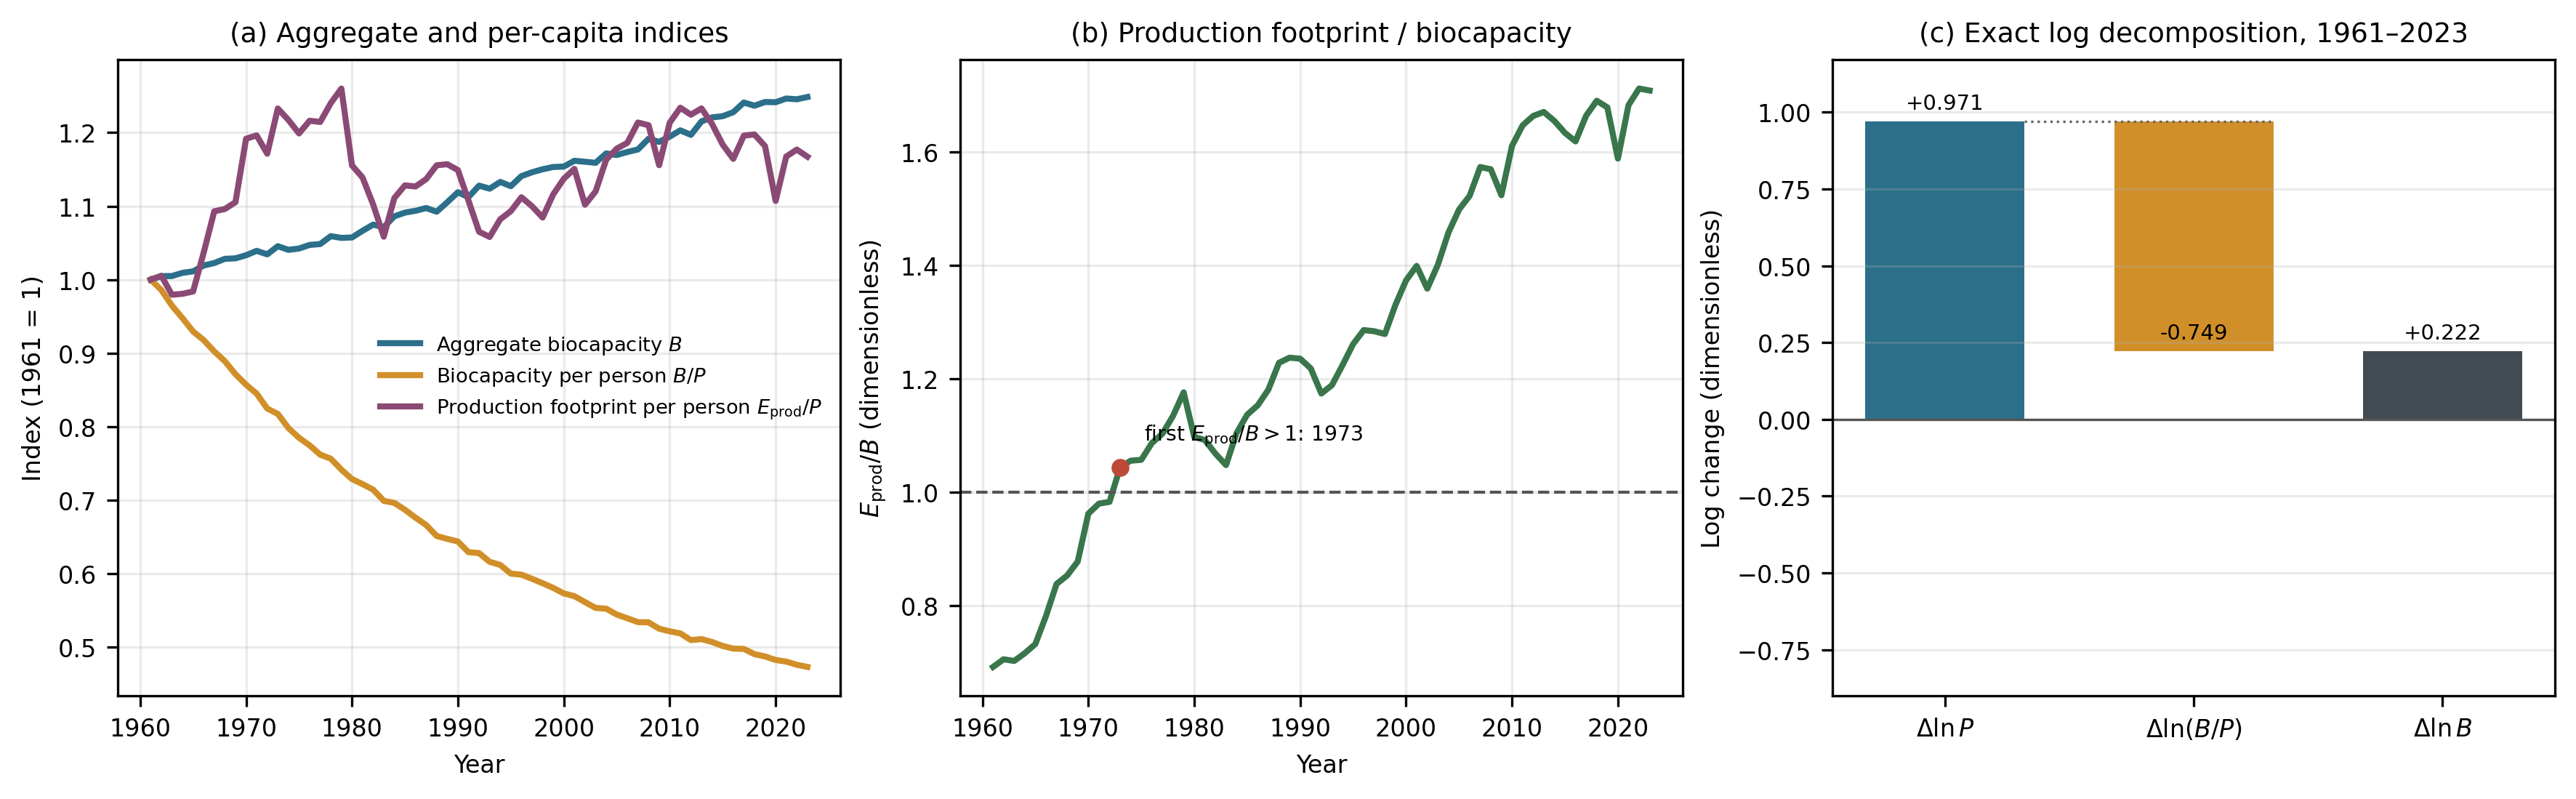
\includegraphics[width=\textwidth]{fig2_nfa_aggregation_face}
\caption{Aggregate and per-capita movements in NFA Edition 2026 (world, 1961--2023; complete observations). $B$ is total biocapacity, $E_{\mathrm{prod}}$ is the workbook's Global Ecological Footprint of Production, and $P$ is the single UN PopStat population series; per-capita values are calculated from totals. (a) Indices (1961 $=1$) of $B$, $B/P$, and $E_{\mathrm{prod}}/P$. (b) $E_{\mathrm{prod}}/B$, first above one in 1973. (c) Exact log identity $\Delta\ln B=\Delta\ln P+\Delta\ln(B/P)$. Account values are in gha; plotted indices, ratios, and log changes are dimensionless. The 2024--2025 estimated rows are excluded.}
\label{fig:aggregation}
\end{figure}

The component series show how NFA account composition changed (Fig.~\ref{fig:composition}; Table~\ref{tab:nfa_components}). Cropland contributes $+24.06$ percentage points to the aggregate's $+24.86\%$ change—about $96.8\%$ of the net percentage change. \mbox{Forest biocapacity} contributes $-5.95$ points, grazing land $-0.27$, fishing grounds $-0.42$, and built-up land $+7.44$. The non-cropland account sum, which includes built-up land, is nearly unchanged ($1.0092\times$, or $+0.80$ points) because the built-up increase offsets declines elsewhere. These are changes in account values. They do not establish changes in forest biomass, soil condition, wetland extent, fish biomass, or model area $A_c$. Built-up land is an account class, not ecological capital. Component values sum to total biocapacity within workbook rounding at both endpoints.

\begin{table}[!htbp]
\centering\footnotesize
\caption{NFA Edition 2026 biocapacity-account endpoint ratios and contributions. Contributions are $100\,[B_i(T)-B_i(1961)]/B(1961)$ percentage points; endpoint ratios are $B_i(T)/B_i(1961)$. The 2022 sensitivity is from the same edition. All entries are account values, not physical-stock measurements.}
\label{tab:nfa_components}
\begin{tabularx}{\textwidth}{@{}Xrrrr@{}}
\toprule
Component & \shortstack{2023\\ratio} & \shortstack{2023 contribution\\(pp of $B_{1961}$)} & \shortstack{2022 sensitivity\\ratio} & \shortstack{2022 contribution\\(pp of $B_{1961}$)} \\
\midrule
Cropland & 2.8701 & $+24.0577$ & 2.8514 & $+23.8183$ \\
Grazing land & 0.9828 & $-0.2688$ & 0.9815 & $-0.2890$ \\
Forest biocapacity & 0.8996 & $-5.9525$ & 0.9019 & $-5.8137$ \\
Fishing grounds & 0.9627 & $-0.4212$ & 0.9596 & $-0.4559$ \\
Built-up land$^{\dagger}$ & 8.7935 & $+7.4416$ & 8.6298 & $+7.2854$ \\
Non-cropland sum$^{\dagger}$ & 1.0092 & $+0.7990$ & 1.0083 & $+0.7267$ \\
\midrule
Total biocapacity & 1.2486 & $+24.8568$ & 1.2454 & $+24.5450$ \\
\bottomrule
\end{tabularx}
\begin{flushleft}\footnotesize
$^{\dagger}$Built-up land is not ecological capital; the non-cropland account sum includes it. Component sums match total biocapacity within workbook rounding. \end{flushleft}
\end{table}

\begin{figure}[!htbp]
\centering
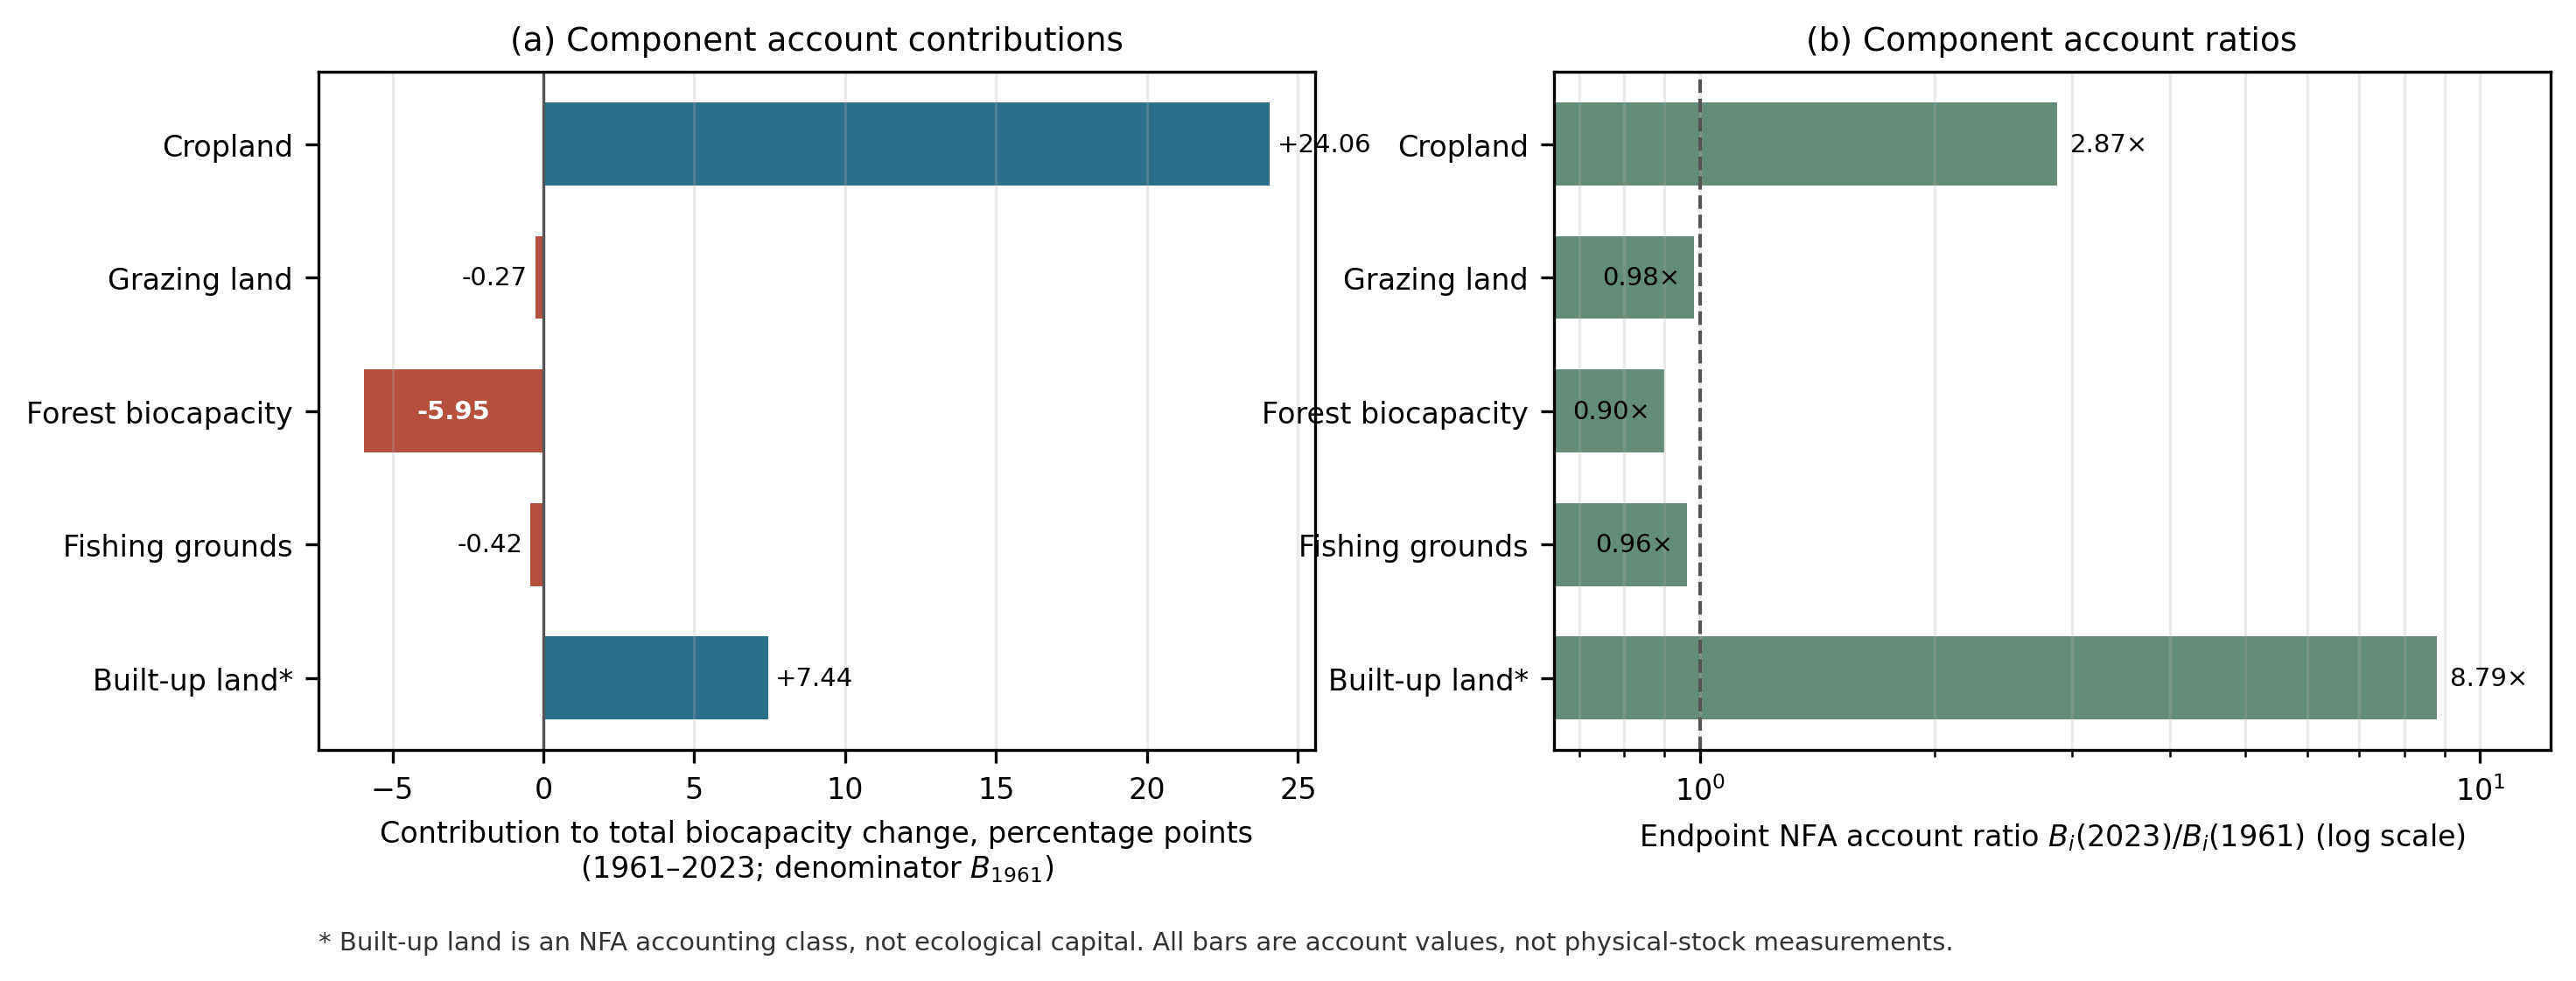
\includegraphics[width=0.95\textwidth]{fig3_composition_attribution}
\caption{NFA Edition 2026 land-type biocapacity-account changes, world, 1961--2023. (a) Component contributions in percentage points of $B_{1961}$. (b) Endpoint ratios $B_i(2023)/B_i(1961)$. “Forest biocapacity” is the workbook's exact label. All bars are account values, not measurements of physical stocks; built-up land is an NFA accounting class, not ecological capital.}
\label{fig:composition}
\end{figure}

We also use external cropland area and cereal yield to build an illustrative proxy for the fast-land contribution (SI~\S S5). Anchoring it to the measured 1961 NFA cropland share ($\phi_0=0.128647$, about $12.86\%$), the exact log-change split assigns $+0.268662$ to the cereal-yield index, $+0.037710$ to cropland area, and $-0.084375$ to the residual. Together these sum to $\Delta\ln B=+0.221997$. The identity is exact for this proxy, but its allocation changes with the anchor and is not a physical-stock attribution.

\subsection{Falsifiable predictions}\label{sec:predictions}

The model yields five testable predictions. Testing its composition mechanism requires more than aggregate biocapacity: it requires information on capital-land area, fast-land area, and relevant land-cover or yield proxies.
\begin{enumerate}[label=P\arabic*.,leftmargin=2.2em]
\item \textbf{Conversion can raise the total under a specific condition.} In the baseline frozen-demand run, $\dot A_c<0$ while $\dot B>0$ for a finite interval (Fig.~\ref{fig:model}a). Conversion adds to $B$ exactly when $\dconv>0$, although other flows, quality, debt, technology, and restoration determine the net change. With baseline shares $\sigma_f=\sigma_c=1$, conversion requires demand to exceed total biocapacity ($R_B=E/B>1$). The reserved-share extension can permit conversion when $R_B\le1$, but that is not a baseline result. A composition mask is rising $B$ with falling $A_c$; a liquidation mask is steady $E$ with falling $A_c$. The two patterns may overlap but are not interchangeable. The sign of $\dconv$ describes conversion's contribution, not necessarily the net change in $B$.
\item \textbf{The duration depends on model rates, not a universal horizon.} The slow return rate $\lambda_1$ (along with $\tconv$, $\mu$, $\eta_f$, and $b_c/b_f$) sets the timescale; $\dconv$ and the initial shortfall affect the size of the change. In the baseline, most conversion occurs within one to two e-folding times, when the remaining gap shrinks by a factor of $e$.
\item \textbf{The reduced model has no fold-type early warning.} Return time does not grow as demand approaches the ceiling, and drawdown depth changes continuously with demand (Fig.~\ref{fig:model}c). The model instead signals that $A_c$ is approaching its minimum. It predicts no fold-related warning before that boundary.
\item \textbf{The population proximity value depends on starting area and is weakly delay-sensitive in the tested range.} The initial population at which a run approaches the capital-land floor rises with starting $A_c$ (Table~\ref{tab:model}b). For $A_{c0}=1.0$\,ha, the $10^{-6}$\,ha proximity value shifts by at most $0.001$\,cap across $\tau_g=5$, $20$, and $40$\,yr (SI Table S2). This comparison does not establish delay invariance beyond that range; the small shift is consistent with the modest regenerative contribution and monotone quality path in the baseline.
\item \textbf{Recovery requires a return flow.} Lower demand alone does not restore capital-land area. The model needs an explicit restoration flow. A surplus-gated flow is inactive during shortfall, whereas a deficit-gated flow can further reduce provision.
\end{enumerate}
Aggregate $B$ alone cannot test these predictions. The composition mechanism requires independent observations or defensible proxies for $A_c$ and fast-land yield $b_f$. Testing delay, recovery, and demand-threshold predictions also requires relevant time series and intervention or demographic data.
\clearpage
\section{Discussion}\label{sec:discussion}

\subsection{What the two-land model shows}

The two-land model yields three results relevant to human--environment models \citep{Schaefer1954,May1973,Meadows1972,Meadows2004,WackernagelRees1996,BranderTaylor1998}. First, conversion can add to total biocapacity while $A_c$ falls. Whether $B$ rises overall also depends on other land flows and quality change; Proposition~\ref{prop:mask} gives the exact condition for the conversion term. The technology boost is capped, while debt depends on the magnitude and duration of shortfall (Proposition~\ref{prop:bounded}).

Second, under the reduced fixed-demand assumptions ($q=q_{\max}$, $D=0$, technology boost off, and no restoration), the balance relation declines steadily with $A_c$ until it meets the area floor. It does not fold back. The absence of a fold, hysteresis, or critical slowing applies to this equilibrium relation, not to every trajectory. With one-way conversion and no return flow, $A_c$ remains below its pre-overshoot level after conversion stops, although it no longer declines at the balance point (Table~\ref{tab:neg}). Third, recovery requires an explicit return flow; its effect depends on whether the restoration gate opens during a shortfall or a surplus.

SI~\S S7 gives a separate one-stock comparator. Its state $A$ has comparator-specific units; it is not $A_c$. With constant parameters and no debt, its equilibrium relation is $B(A)=(b+b_G\rho)A-(b_G\rho/A_{\max})A^2$, with $P=B(A)/e$. At the illustrated settings, $b_G\rho<b$, so the relation is monotone; an interior maximum would require other parameters. Its neutral equilibrium family and selected delay trajectories belong only to that formulation. They establish neither a fold nor a universal critical delay or collapse mechanism in the two-land model.

These results also clarify when to expect common early-warning indicators. Rising autocorrelation and variance are associated with approaching a fold \citep{Scheffer2001}. This reduced model reaches a minimum-area boundary instead, so those indicators need not rise first. Their absence would not establish safety. The relevant model signal is the path of $A_c$, which the aggregate alone cannot reveal.

\begin{table}[!htbp]
\centering\footnotesize
\caption{Equilibrium, trajectory, and tested delay-sensitivity properties under the stated assumptions.}
\label{tab:neg}
\begin{tabularx}{\textwidth}{>{\raggedright\arraybackslash}p{0.34\textwidth} l >{\raggedright\arraybackslash}X}
\toprule
Property & Finding & Scope \\
\midrule
Fold on the reduced frozen-demand branch & Absent & $B_{eq}(A_c)$ is strictly monotone; the balance point collides with the typed floor at $\Eceil\approx1.138\,\mathrm{gha}$ (Proposition~\ref{prop:ceiling}) \\
Critical slowing as $E\to\Eceil$ & Absent & The slow eigenvalue remains negative and constant along the reduced branch \\
Hysteresis of the frozen-demand equilibrium relation & Absent & There is at most one feasible balance point; this does not imply history independence of realized states \\
Path dependence of realized $A_c$ & Present, conditional & With $R_{rc}=0$, one-way conversion leaves $A_c$ below its pre-overshoot level after shortfall closure, while $\dot A_c=0$ at equilibrium \\
Discontinuous response to endogenous demand & Not observed & In the reported runs, minimum $A_c$ varies continuously and monotonically with initial population; proximity thresholds depend on tolerance \\
Regeneration-delay sensitivity ($\tau_g$, with $\tau_p=25$\,yr) & Small in tested range & At $A_{c0}=1.0$\,ha, the delayed-quality $10^{-6}$\,ha threshold varies by $0.001$\,cap across $\tau_g=5,20,40$\,yr (SI Table S2); this does not establish invariance outside that range \\
\bottomrule
\end{tabularx}
\end{table}
\clearpage

\subsection{Measurement implications}

Biocapacity in gha is a value-weighted total, not an inventory of land classes. A $20\%$ increase cannot distinguish modest gains across all components from a large gain in one that offsets losses elsewhere. Proposition~\ref{prop:mask}(iii) formalizes the limit: even with fixed per-hectare yields, the total and the conserved-area constraint leave multiple feasible allocations among fast, capital, and reserve land.

A related transition-assessment study defines a linear compensatory operator and compares perfect substitutability with less-substitutable CES alternatives \citep[Sections~2 and 4 of][]{Abaee2026b}. ECOMOD's $B$ is also a linear sum, but the companion analyzes a different, finite-plan setting. There, the compensatory protocol accepts states even when no single available plan meets every component floor (Theorem~2 in \citet{Abaee2026b}). Theorem~4(iii) in \citet{Abaee2026b} identifies an exact interval of diagonal-gap states on its witness-defined region that each positive elasticity falsely certifies as safe; thus no positive-elasticity member is uniformly safe on that region. If feasibility is required throughout a transition, falling below a land-class minimum remains a violation even if the endpoint later recovers.

For the NFA, these findings concern account composition, not physical stocks. In Edition 2026, total world biocapacity account value $B$ rises $24.86\%$ from 1961 to 2023, while $B/P$ falls $52.71\%$. The Global Ecological Footprint of Production per person ($E_{\mathrm{prod}}/P$) rises $16.73\%$, and $E_{\mathrm{prod}}/B$ first exceeds one in 1973. $B$ and $E_{\mathrm{prod}}$ are annual account amounts in gha, with the annual basis implicit; per-person values are in gha per person, and $E_{\mathrm{prod}}/B$ is dimensionless.

Cropland contributes $+24.06$ percentage points to the total change; Forest biocapacity contributes $-5.95$, grazing land $-0.27$, fishing grounds $-0.42$, and built-up land $+7.44$. The non-cropland sum is nearly flat because these account movements offset one another, including the large built-up-land increase. SI~\S S5 reports the same-edition 1961--2022 comparison. None of these values measures forest biomass or condition, soil carbon, wetland extent, fish biomass, or another physical stock. In particular, a decline in Forest biocapacity does not establish a decline in forest biomass. Built-up land is an NFA accounting class, not ecological capital. The ratios, contributions, vintage, and endpoint sensitivity describe account composition only \citep{Lo2026NFA,Borucke2013,Blomqvist2013,GiampietroSaltelli2014,Galli2016,vdBerghGrazi2015}.

The model result is distinct from the NFA trends. In the frozen-demand baseline (Fig.~\ref{fig:model}a), $A_c$ falls from $1.500$ to $0.807659$\,ha ($46.16\%$), while model $B$ rises from $0.594$ to $0.825$\,gha ($39\%$). Quality $q$ rises from $0.9$ to $1.0$, moving farther above $q^*=q_{\max}/2$, where $\Ups(q)$ peaks. Its per-hectare value therefore falls from $0.05576$ to $0.05000$\,gha\,ha$^{-1}$ ($10.33\%$), and the modeled contribution $\Ups(q)A_c$ falls from $0.08364$ to $0.04038$\,gha ($51.72\%$).

With restoration off, one-way conversion leaves $A_c$ below its starting value after the shortfall closes. It then remains at the lower balance level rather than declining indefinitely. This is a conditional model result, not an observation or estimate of global physical-stock change.

We assembled no common-boundary global physical-stock series for these components and therefore report no physical-stock composite or global decline finding. The SI scoreboard is a specification—not an inventory—with candidate stock, extent, condition, and annual-flow measures and the requirements for comparing them; it contains no endpoint values. Until spatial and temporal boundaries, units, uncertainty, overlap, valuation or normalization, and permitted substitution are specified, these unlike measures should remain a nonadditive vector. SEEA Ecosystem Accounting also reports ecosystem extent and condition separately from ecosystem services and monetary presentations \citep{UN2021SEEA_EA}.

The external cropland-area and cereal-yield series provide an illustrative proxy, not direct measurements of the model's land classes. The proxy is anchored to the 1961 NFA cropland share; cereal yield is a productivity sentinel, not an all-crops measure, and the area and account boundaries do not match by construction. External cropland area $A_f$ is in hectares and index-scaled yield $\hat b_f$ in gha\,ha$^{-1}$, so $X=\hat b_fA_f$ and $C=B-X$ are account amounts in gha. The residual can absorb boundary and calibration differences, other account components, and conversion-factor changes. It is neither $\Ups(q)A_c$ nor a physical-stock measure. Physical interpretation would require independent, boundary-consistent measures of area, condition, yield, and regeneration, together with a validated mapping and valuation. Forest area could inform one part of the effective capital class, but cannot represent the entire class or its condition.

\subsection{Policy controls and limits}

We compare three controls. A conversion stop triggered at $A_c=\Acmin$ preserves the capital-land floor. A ceiling on fast-land area $A_f$ does not guarantee that floor unless the stop rule is explicitly tied to it and to the remaining-area constraints. Nor can a heuristic governor that monitors only total $B$ guarantee the floor: the aggregate does not identify $A_c$.

The restoration gates also behave differently. Surplus-gated restoration is inactive during a shortfall; deficit-gated restoration acts during the shortfall and can reduce provision further. This comparison echoes the distinction between protective and mobilizing institutional feedback in related work \citep{Abaee2026a}. With a common reserved share, $\sigma_f=\sigma_c=\sigma<1$, conversion is inactive while $E\le\sigma B$. With separate shares, the condition is $E\le\sigma_fY_f+\sigma_cY_c$. This reservation applies to annual human-available flow, not to spatially protected area. Half-Earth, by contrast, is a spatial conservation target \citep{Wilson2016}. The connection is only the abstract idea of reservation: the model neither maps protected areas nor evaluates that proposal. Robustness to disturbances and parameter uncertainty remains untested.

\subsection{Relation to prior work}

The ledger companion distinguishes weak and strong sustainability as operating regimes according to whether material loops close at throughput. In its terms, a positive weighted sum ranks outcomes under weak sustainability, whereas componentwise adequacy is the strong-sustainability predicate \citep[Sections~1.1 and 10.1]{Abaee2026c}. ECOMOD's $B$ is an annual biocapacity-account total. The link is an analogy about compensation, not an identity with the companion's material-flow ledger or a complete sustainability classification. The assessment companion studies aggregate measures and typed transition criteria in a separate finite-plan setting \citep{Abaee2026b}; the governance companion studies institutional feedback \citep{Abaee2026a}. The delays here represent ecological regeneration and demographic response, not institutional review.

\subsection{Limitations}

Several limitations set the scope of the results. Ecological-capital land combines unlike assets, so its single quality state, regeneration rule, composition diagnostic, and demand ceiling are effective model quantities—not estimates for forests, soils, or wetlands. Most parameters are representative rather than fitted. A cross-section cannot identify $b_c$, $b_{G,c}$, and $\rho_c$ separately. Recovery records from different systems provide timescale context, not a global estimate of $\rho_c$; they describe regeneration responses, not the delay $\tau_g$. We hold the per-person footprint constant to isolate feedbacks among land, biocapacity, and demand. A changing footprint would require another model extension.

The composition pattern depends on demand and on the mechanisms included here; under the stated assumptions, it is bounded. The exact shortfall switch makes stability at $S=0$ one-sided. Drawdown thresholds are reported as proximity bands because they depend on tolerance and time step. We fix debt repayment at $\eta=0.05$\,yr$^{-1}$; the zero-repayment limit ($\eta\to0$), which removes the debt equilibrium, is not analyzed. NFA accounts combine area and yield and therefore cannot identify them separately. Finally, replacing delayed regeneration $G_c(q(t-\tau_g))$ with current-quality regeneration $G_c(q(t))$ lengthens the demonstration mask by $1.3$\,yr and shifts the initial-population threshold by at most $0.001$\,cap (SI~\S S3).

\section{Conclusions}\label{sec:conclusions}

An aggregate biocapacity total does not reveal how its land classes change. In the two-land model, conversion adds to $B$ when fast-land yield exceeds capital land's effective per-hectare value, even as $A_c$ falls; other terms determine whether $B$ rises overall (Proposition~\ref{prop:mask}). Under the reduced fixed-demand assumptions, the balance relation has one branch and reaches the area floor without a fold, hysteresis, or critical slowing. Realized paths remain history-dependent: with restoration off, $A_c$ stays below its pre-overshoot level after the shortfall closes, but does not keep falling at the balance point. In the representative run, $A_c$ falls $46.16\%$, $\Ups(q)$ falls $10.33\%$, and $\Ups(q)A_c$ falls $51.72\%$, while model $B$ rises $39\%$. These are conditional model results, not estimates of global physical stocks.

In NFA Edition 2026, total world biocapacity account value rises $24.86\%$ from 1961 to 2023, while $B/P$ falls $52.71\%$ and the production footprint per person rises $16.73\%$. Cropland contributes $24.06$ percentage points to the account total; Forest biocapacity subtracts $5.95$ points, and built-up land contributes $+7.44$ as an accounting class—not ecological capital. These movements do not measure biomass, soil condition, wetland extent, fish biomass, or $A_c$. The 1961--2022 sensitivity uses the same account edition and population series. No common-boundary global physical-stock series was assembled, so we report no composite or global decline finding. The SI scoreboard specifies candidate measures and comparison requirements; it is not an empirical inventory. Until boundaries, units, uncertainty, overlap, valuation or normalization, and allowed substitution are specified, physical measures remain a nonadditive vector. The proxy residual $C=B-\hat b_fA_f$ is neither a physical-capital measure nor the model contribution $\Ups(q)A_c$. A future comparison would require independent observations and a validated mapping.

The practical lesson is simple: report component accounts alongside the aggregate. The orchard is a metaphor for the information problem, not evidence of a measured global stock decline. One record tracks the annual harvest; another would need independent, comparable observations of the trees, soil, and other assets that support future harvests. That physical record cannot be inferred from the account total. A harvest total is not a census of the orchard.

\section*{Acknowledgments}

The author thanks Global Footprint Network for making its data publicly available; Mathis Wackernagel for his thoughtful review; the editors of \emph{Ecological Modelling} for their trust and support; and Arena.ai for its ingenuity and online tools.

\section*{Declarations}

\paragraph{Data availability} All empirical inputs are publicly available from the sources cited in the manuscript. Derived analysis data and model code will be deposited in a public GitHub repository and archived in Zenodo; repository and record details will be added after the deposit is complete.

\paragraph{Funding} No funding was received.

\paragraph{Competing interests} The author declares no competing interests.

\paragraph{CRediT authorship contribution statement} \textbf{Amin Abaee:} Conceptualization; Methodology; Software; Formal analysis; Writing -- original draft; Writing -- review \& editing.

\paragraph{Declaration of generative AI in scientific writing} DeepSeek AI and Claude (Anthropic) assisted with computational-reproducibility checks under the author's supervision; the author reviewed and edited the content and takes full responsibility for the publication.
\begin{thebibliography}{99}
\bibitem[{Abaee(2026a)}]{Abaee2026a} Abaee, A. (2026a). \emph{Governance delay and the stability of harvested stocks: mobilising and protective feedback rules, and the review interval as a design parameter}. Working paper (v41). \url{https://github.com/MIKEAA2020/general-sustainability/blob/2efaa62083f2007dec3446c15c475af88f0925f3/arena%20agent%201/paper%20rewrites/latex/paper4_delay_dynamics_v41.pdf}.
\bibitem[{Abaee(2026b)}]{Abaee2026b} Abaee, A. (2026b). \emph{Aggregation is a claim, not a presentation: the geometry of the acceptance gap between compensatory and noncompensatory transition assessment}. Working paper (v71). \url{https://github.com/MIKEAA2020/general-sustainability/blob/2efaa62083f2007dec3446c15c475af88f0925f3/arena%20agent%201/paper%20rewrites/latex/paper06_assessment_separation_v71.pdf}.
\bibitem[{Abaee(2026c)}]{Abaee2026c} Abaee, A. (2026c). \emph{Typed Flux Ledgers and Depletion Arithmetic: Conservation, Componentwise Diagnostics, and the Semantics of Depletion Horizons}. Working paper. PDF pinned to GitHub commit \url{https://github.com/MIKEAA2020/general-sustainability/blob/2efaa62083f2007dec3446c15c475af88f0925f3/paper3/latest-2026-09-19/manuscript/paper3_material_ledgers_v50.pdf}.
\bibitem[{Anderies(2000)}]{Anderies2000} Anderies, J. M. (2000). On modeling human behavior and institutions in simple ecological economic systems. \emph{Ecological Economics}, 35(3), 393--412.
\bibitem[{Becker et al.(2017)}]{Becker2017} Becker, W., Saisana, M., Paruolo, P. \& Vandecasteele, I. (2017). Weights and importance in composite indicators: Closing the gap. \emph{Ecological Indicators}, 80, 12--22.
\bibitem[{Blomqvist et al.(2013)}]{Blomqvist2013} Blomqvist, L., Brook, B. W., Ellis, E. C., Kareiva, P. M., Nordhaus, T. \& Shellenberger, M. (2013). Does the shoe fit? Real versus imagined ecological footprints. \emph{PLoS Biology}, 11(11), e1001700.
\bibitem[{Borucke et al.(2013)}]{Borucke2013} Borucke, M., Moore, D., Cranston, G., Gracey, K., Iha, K., Larson, J., Lazarus, E., Morales, J. C., Wackernagel, M. \& Galli, A. (2013). Accounting for demand and supply of the biosphere's regenerative capacity: The National Footprint Accounts' underlying methodology and framework. \emph{Ecological Indicators}, 24, 518--533.
\bibitem[{Brander and Taylor(1998)}]{BranderTaylor1998} Brander, J. A. \& Taylor, M. S. (1998). The simple economics of Easter Island: A Ricardo--Malthus model of renewable resource use. \emph{American Economic Review}, 88(1), 119--138.
\bibitem[{Calvin and Bond-Lamberty(2018)}]{CalvinBondLamberty2018} Calvin, K. \& Bond-Lamberty, B. (2018). Integrated human--Earth system modeling --- state of the science and future directions. \emph{Environmental Research Letters}, 13(6), 063006.
\bibitem[{Cohen(1995)}]{Cohen1995} Cohen, J. E. (1995). Population growth and Earth's human carrying capacity. \emph{Science}, 269(5222), 341--346.
\bibitem[{Dasgupta(2021)}]{Dasgupta2021} Dasgupta, P. (2021). \emph{The Economics of Biodiversity: The Dasgupta Review.} London: HM Treasury.
\bibitem[{Donges et al.(2017)}]{Donges2017} Donges, J. F., Winkelmann, R., Cornell, S. E., Lucht, W., Dyke, J. G., Rockstr\"om, J., Heitzig, J. \& Schellnhuber, H. J. (2017). Closing the loop: Reconnecting human dynamics to Earth system science. \emph{The Anthropocene Review}, 4(2), 151--157.
\bibitem[{Erb et al.(2017)}]{Erb2017} Erb, K.-H., Luyssaert, S., Meyfroidt, P., Pongratz, J., Don, A., Kloster, S., Kuemmerle, T., Fetzel, T., Fuchs, R., Hasegawa, T., Haberl, H., et al. (2017). Land management: data availability and process understanding for global change studies. \emph{Global Change Biology}, 23(2), 512--533.
\bibitem[{Fischer et al.(2022)}]{Fischer2022} Fischer, S. M., Joy, M. K., Abrahamse, W., Milfont, T. L. \& Petherick, L. M. (2022). The use and misuse of composite environmental indices. \emph{bioRxiv}, 2022.03.15.484501. \url{https://doi.org/10.1101/2022.03.15.484501}.
\bibitem[{Global Footprint Network(2009)}]{GFNStandards2009} Global Footprint Network (2009). \emph{Ecological Footprint Standards 2009}. Global Footprint Network. \url{https://www.footprintnetwork.org/content/uploads/2019/05/Ecological_Footprint_Standards_2009.pdf}.
\bibitem[{Global Footprint Network(2019)}]{GFNGuidebook2019} Global Footprint Network (2019). \emph{Working Guidebook to the National Footprint Accounts 2019}. Global Footprint Network. \url{https://www.footprintnetwork.org/content/uploads/2019/05/National_Footprint_Accounts_Guidebook_2019.pdf}.
\bibitem[{Galli et al.(2016)}]{Galli2016} Galli, A., Giampietro, M., Goldfinger, S., Lazarus, E., Lin, D., Saltelli, A., Wackernagel, M. \& M\"uller, F. (2016). Questioning the ecological footprint. \emph{Ecological Indicators}, 69, 224--232.
\bibitem[{Giampietro and Saltelli(2014)}]{GiampietroSaltelli2014} Giampietro, M. \& Saltelli, A. (2014). Footprints to nowhere. \emph{Ecological Indicators}, 46, 610--621.
\bibitem[{Haberl et al.(2007)}]{Haberl2007} Haberl, H., Erb, K.-H., Krausmann, F., Gaube, V., Bondeau, A., Plutzar, C., Gingrich, S., Lucht, W. \& Fischer-Kowalski, M. (2007). Quantifying and mapping the human appropriation of net primary production in earth's terrestrial ecosystems. \emph{PNAS}, 104(31), 12942--12947.
\bibitem[{Henderson and Loreau(2018)}]{HendersonLoreau2018} Henderson, K. \& Loreau, M. (2018). How ecological feedbacks between human population and land cover influence sustainability. \emph{PLoS Computational Biology}, 14(8), e1006389.
\bibitem[{Hutchings and Reynolds(2004)}]{HutchingsReynolds2004} Hutchings, J. A. \& Reynolds, J. D. (2004). Marine fish population collapses: consequences for recovery and extinction risk. \emph{BioScience}, 54(4), 297--309.
\bibitem[{Hutchinson(1948)}]{Hutchinson1948} Hutchinson, G. E. (1948). Circular causal systems in ecology. \emph{Annals of the New York Academy of Sciences}, 50(4), 221--246.
\bibitem[{Krausmann et al.(2013)}]{Krausmann2013} Krausmann, F., Erb, K.-H., Gingrich, S., Haberl, H., Bondeau, A., Gaube, V., Lauk, C., Plutzar, C. \& Searchinger, T. D. (2013). Global human appropriation of net primary production doubled in the 20th century. \emph{PNAS}, 110(25), 10324--10329.
\bibitem[{Lo et al.(2026)}]{Lo2026NFA} Lo, K., Basnet, N., Miller, E., Srikanthalingam, B., Foley, B., Van Berkum, J. L., Long, A. H., Toneva, P., Ermina, M. \& Klinkenberg, C. (2026). \emph{National Ecological Footprint and Biocapacity Accounts, Edition 2026 (1961--2025): Results and metadata, version 1.0.} Prepared for Footprint Data Foundation by researchers at York University and the University of Iceland. Workbook: \url{https://footprint.info.yorku.ca/files/2026/04/NEFBA_Data_global_national_ecological_footprint_biocapacity.xlsx}; release notes: \url{https://footprint.info.yorku.ca/files/2026/04/NEFBA_ReleaseNotes.pdf}; data page: \url{https://footprint.info.yorku.ca/data/}.
\bibitem[{May(1973)}]{May1973} May, R. M. (1973). \emph{Stability and Complexity in Model Ecosystems.} Princeton: Princeton University Press.
\bibitem[{Meadows et al.(1972)}]{Meadows1972} Meadows, D. H., Meadows, D. L., Randers, J. \& Behrens, W. W. (1972). \emph{The Limits to Growth.} New York: Universe Books.
\bibitem[{Meadows et al.(1974)}]{Meadows1974} Meadows, D. L., Behrens, W. W., Meadows, D. H., Naill, R. F., Randers, J. \& Zahn, E. (1974). \emph{Dynamics of Growth in a Finite World.} Cambridge, MA: Wright-Allen Press.
\bibitem[{Meadows et al.(2004)}]{Meadows2004} Meadows, D. H., Randers, J. \& Meadows, D. L. (2004). \emph{The Limits to Growth: The 30-Year Update.} White River Junction, VT: Chelsea Green.
\bibitem[{Meyer(1994)}]{Meyer1994} Meyer, P. S. (1994). Bi-logistic growth. \emph{Technological Forecasting and Social Change}, 47(1), 89--102.
\bibitem[{Meyer and Ausubel(1999)}]{MeyerAusubel1999} Meyer, P. S. \& Ausubel, J. H. (1999). Carrying capacity: A model with logistically varying limits. \emph{Technological Forecasting and Social Change}, 61(3), 209--214.
\bibitem[{Motesharrei et al.(2016)}]{Motesharrei2016} Motesharrei, S., Rivas, J., Kalnay, E., Asrar, G. R., Busalacchi, A. J., Cahalan, R. F., Cane, M. A., Colwell, R. R., Feng, K., Franklin, R. S., et al. (2016). Modeling sustainability: Population, inequality, consumption, and bidirectional coupling of the Earth and human systems. \emph{National Science Review}, 3(4), 470--494.
\bibitem[{Nardo et al.(2008)}]{Nardo2008} Nardo, M., Saisana, M., Saltelli, A., Tarantola, S., Hoffmann, A. \& Giovannini, E. (2008). \emph{Handbook on Constructing Composite Indicators: Methodology and User Guide.} Paris: OECD Publishing.
\bibitem[{Neubauer et al.(2013)}]{Neubauer2013} Neubauer, P., Jensen, O. P., Hutchings, J. A. \& Baum, J. K. (2013). Resilience and recovery of overexploited marine populations. \emph{Science}, 340(6130), 347--349.
\bibitem[{Our~World~in~Data(2026a)}]{OWIDCereal2026} Our~World~in~Data (2026a). \emph{Cereal yield.} FAOSTAT data accessed through Our World in Data; grapher page last updated 25 February 2026; accessed 24 October 2026. \url{https://ourworldindata.org/grapher/cereal-yield}.
\bibitem[{Our~World~in~Data(2026b)}]{OWIDCropland2026} Our~World~in~Data (2026b). \emph{Cropland area.} FAOSTAT data accessed through Our World in Data; grapher page last updated 25 February 2026; accessed 24 October 2026. \url{https://ourworldindata.org/grapher/cropland-area}.
\bibitem[{Pearl(1925)}]{Pearl1925} Pearl, R. (1925). \emph{The Biology of Population Growth.} New York: Alfred A. Knopf.
\bibitem[{Poeplau et al.(2011)}]{Poeplau2011} Poeplau, C., et al. (2011). Temporal dynamics of soil organic carbon after land-use change in the temperate zone--carbon response functions as a model approach. \emph{Global Change Biology}, 17(7), 2415--2427.
\bibitem[{Poorter et al.(2016)}]{Poorter2016} Poorter, L., et al. (2016). Biomass resilience of Neotropical secondary forests. \emph{Nature}, 530(7590), 211--214.
\bibitem[{Schaefer(1954)}]{Schaefer1954} Schaefer, M. B. (1954). Some aspects of the dynamics of populations important to the management of the commercial marine fisheries. \emph{Bulletin of the Inter-American Tropical Tuna Commission}, 1(2), 25--56.
\bibitem[{Scheffer et al.(2001)}]{Scheffer2001} Scheffer, M., Carpenter, S., Foley, J. A., Folke, C. \& Walker, B. (2001). Catastrophic shifts in ecosystems. \emph{Nature}, 413(6856), 591--596.
\bibitem[{Simon(1996)}]{Simon1996} Simon, J. L. (1996). \emph{The Ultimate Resource 2.} Princeton: Princeton University Press.
\bibitem[{United Nations et al.(2021)}]{UN2021SEEA_EA} United Nations et al. (2021). \emph{System of Environmental-Economic Accounting---Ecosystem Accounting (SEEA EA).} White cover publication, pre-edited text subject to official editing. New York: United Nations. \url{https://seea.un.org/ecosystem-accounting}.
\bibitem[{United Nations(2022)}]{UN2022} United Nations (2022). \emph{World Population Prospects 2022: Summary of Results.} New York: Department of Economic and Social Affairs, Population Division.
\bibitem[{van den Bergh and Grazi(2015)}]{vdBerghGrazi2015} van den Bergh, J. C. J. M. \& Grazi, F. (2015). Reply to the first systematic response by the Global Footprint Network to criticism: a real debate finally? \emph{Ecological Indicators}, 58, 458--463.
\bibitem[{van den Bergh and Rietveld(2004)}]{vdBerghRietveld2004} van den Bergh, J. C. J. M. \& Rietveld, P. (2004). Reconsidering the limits to world population: Meta-analysis and meta-prediction. \emph{BioScience}, 54(3), 195--204.
\bibitem[{Wackernagel and Rees(1996)}]{WackernagelRees1996} Wackernagel, M. \& Rees, W. (1996). \emph{Our Ecological Footprint: Reducing Human Impact on the Earth.} New Society Publishers.
\bibitem[{Wilson(2016)}]{Wilson2016} Wilson, E. O. (2016). \emph{Half-Earth: Our Planet's Fight for Life.} New York: Liveright.
\end{thebibliography}

\end{document}
